% 1.1.3. Disk graphs and problem definitions

% For the sake of simplicity, throughout this thesis we often refer to disks and their corre- sponding vertices synonymously. For example, we might simply say ’we create a disk D2 with radius r2 that touches disk D1’ instead of saying ’we create a vertex v2, a correspond- ing disk D2 with radius r2 and an edge between v2 and vertex v1 whose corresponding disk is D1’.
% Let G = (V, E) be a graph. We say that G has a realization as a disk intersection (touching) graph, if there exist a set of disks V and a bijection from V to V such that G = (G,V) is a disk intersection (touching) graph. In this case, we say G realizes G. Let Dv ∈ V be the disk of G corresponding to vertex v for any v ∈ V . A radius assignment for G is a function r : V → R+ that assigns a positive real number to each vertex of G. If the radius of disk Dv ∈ V is equal to r(v) for every v ∈ V , then G is said to respect r. A seed assignment for G is a function σ : V → R2 that assigns a point in the plane to each vertex ofG.Ifσ(v)∈Dv foreveryv∈V,thenGissaidtorespectσ.LetΓbeacombinatorial embedding for G. If G is a disk touching graph and if the cyclic order of disks touched by Dv corresponds to the cyclic order of edges incident to the vertex v for any v ∈ V , then G is said to respect Γ.
% We consider the following family of decision problems, in which the dots (...) are a place- holder for one, multiple or none of the enlisted variants.
% (Unit/ρ-bounded) Disk Intersection/Touching Graph Recognition (with ...): The problem instance is a graph G = (V, E) and the question is whether it is possible to realize G as a (unit/ρ-bounded) disk intersection/touching graph (which respects ...).
% • ... fixed Radii: ... a given radius assignment r for G.
% • ... fixed Embedding: ... a given combinatorial embedding Γ for G. • ... fixed Seeds: ... a given seed assignment σ for G.
% In particular, we consider the following problems:
% • Unit Disk Touching Graph Recognition (UDT)
% • Unit Disk Touching Graph Recognition with fixed Embedding (UDTE)
% • ρ-bounded Disk Touching Graph Recognition (ρ-BDT)
% • Disk Touching Graph Recognition with fixed Radii (DTR)
% • Disk Touching Graph Recognition with fixed Radii and Embedding (DTRE)
% • Disk Touching Graph Recognition with fixed Seeds (DTS)
% • Unit Disk Touching Graph Recognition with fixed Seeds (UDTS)
% • Unit Disk Touching Graph Recognition with fixed Seeds and Embedding (UDTSE)
% 1.2. Related work
% As mentioned in the beginning of this chapter, Koebe’s Theorem [Koe36] implies that the Disk Touching Graph Recognition problem can be solved in linear time. On the other hand, Hlinˇeny ́ and Kratochv ́ıl showed that the Disk Intersection Graph Recognition problem is NP-hard [HK01].
% A result by Breu and Kirkpatrick states that the Unit Disk Intersection/Touching Graph Recognition problems are NP-hard [BK98], implying that the Disk Intersection/Touching Graph Recognition with fixed Radii problems are also N P -hard. There exists some heuris- tics for generating disk touching graphs with fixed radii [Dor96, Ino11] for the application of cartogram generation.
% 6
% Breu and Kirkpatrick generalized their results by showing that the ρ-bounded Disk Inter- section/Touching Graph Recognition problems are NP-hard for any fixed ρ ≥ 1 [BK96]. Alam et al. [AEG+14] argue that for any tree, for any cactus (which is a connected graph in which each edge is contained in at most one cycle), for any k-outerplanar graph with bounded maximum degree and k ∈ O(log n) and for any planar graph with bounded tree- depth there exists a realizing ρ-bounded disk touching graph where ρ is a polynomial in the number of vertices.
% Atienza et al. show that the Disk Touching Graph Recognition with fixed Seeds problem is NP-hard [AdCC+12].








\section{Disk Arrangements}
%Circle packing theorem: For every connected simple planar graph G there is a circle packing in the plane whose intersection graph is (isomorphic to) G.
% A disk D is a region in the plane bounded by a circle. A disk can be uniquely described by its bounding circle’s radius r ∈ R+ and center c ∈ R2. A disk is called closed if it contains the points of its bounding circle and open otherwise. A disk intersection graph G = (G, V) consists of a graph G = (V,E), a set of closed disks V and a bijection from the set of vertices V to V such that two vertices of V are adjacent in G if and only if their corresponding disks in V intersect. A disk touching graph G = (G, V) is a disk intersection graph such that the interiors of the disks in V are pairwise disjoint. The centers of the disks in V together with straight-line segments that connect the centers of all pairs of touching disks induce a planar drawing of G. In a unit disk intersection (touching) graph all disks share one uniform radius. In a ρ-bounded disk intersection (touching) graph the radius of all disks is taken from the interval [1, ρ] for a value ρ ≥ 1. Note, that a 1-bounded disk intersection (touching) graph is a unit disk intersection (touching) graph.





 A \textit{disk arrangement} is a set of interior disjoint disks, $D$.  
 If for any pair of disks in $D$ intersect at a boundary point, they are said to be in contact (kissing).
\begin{figure}[!hbtp]
\begin{center}
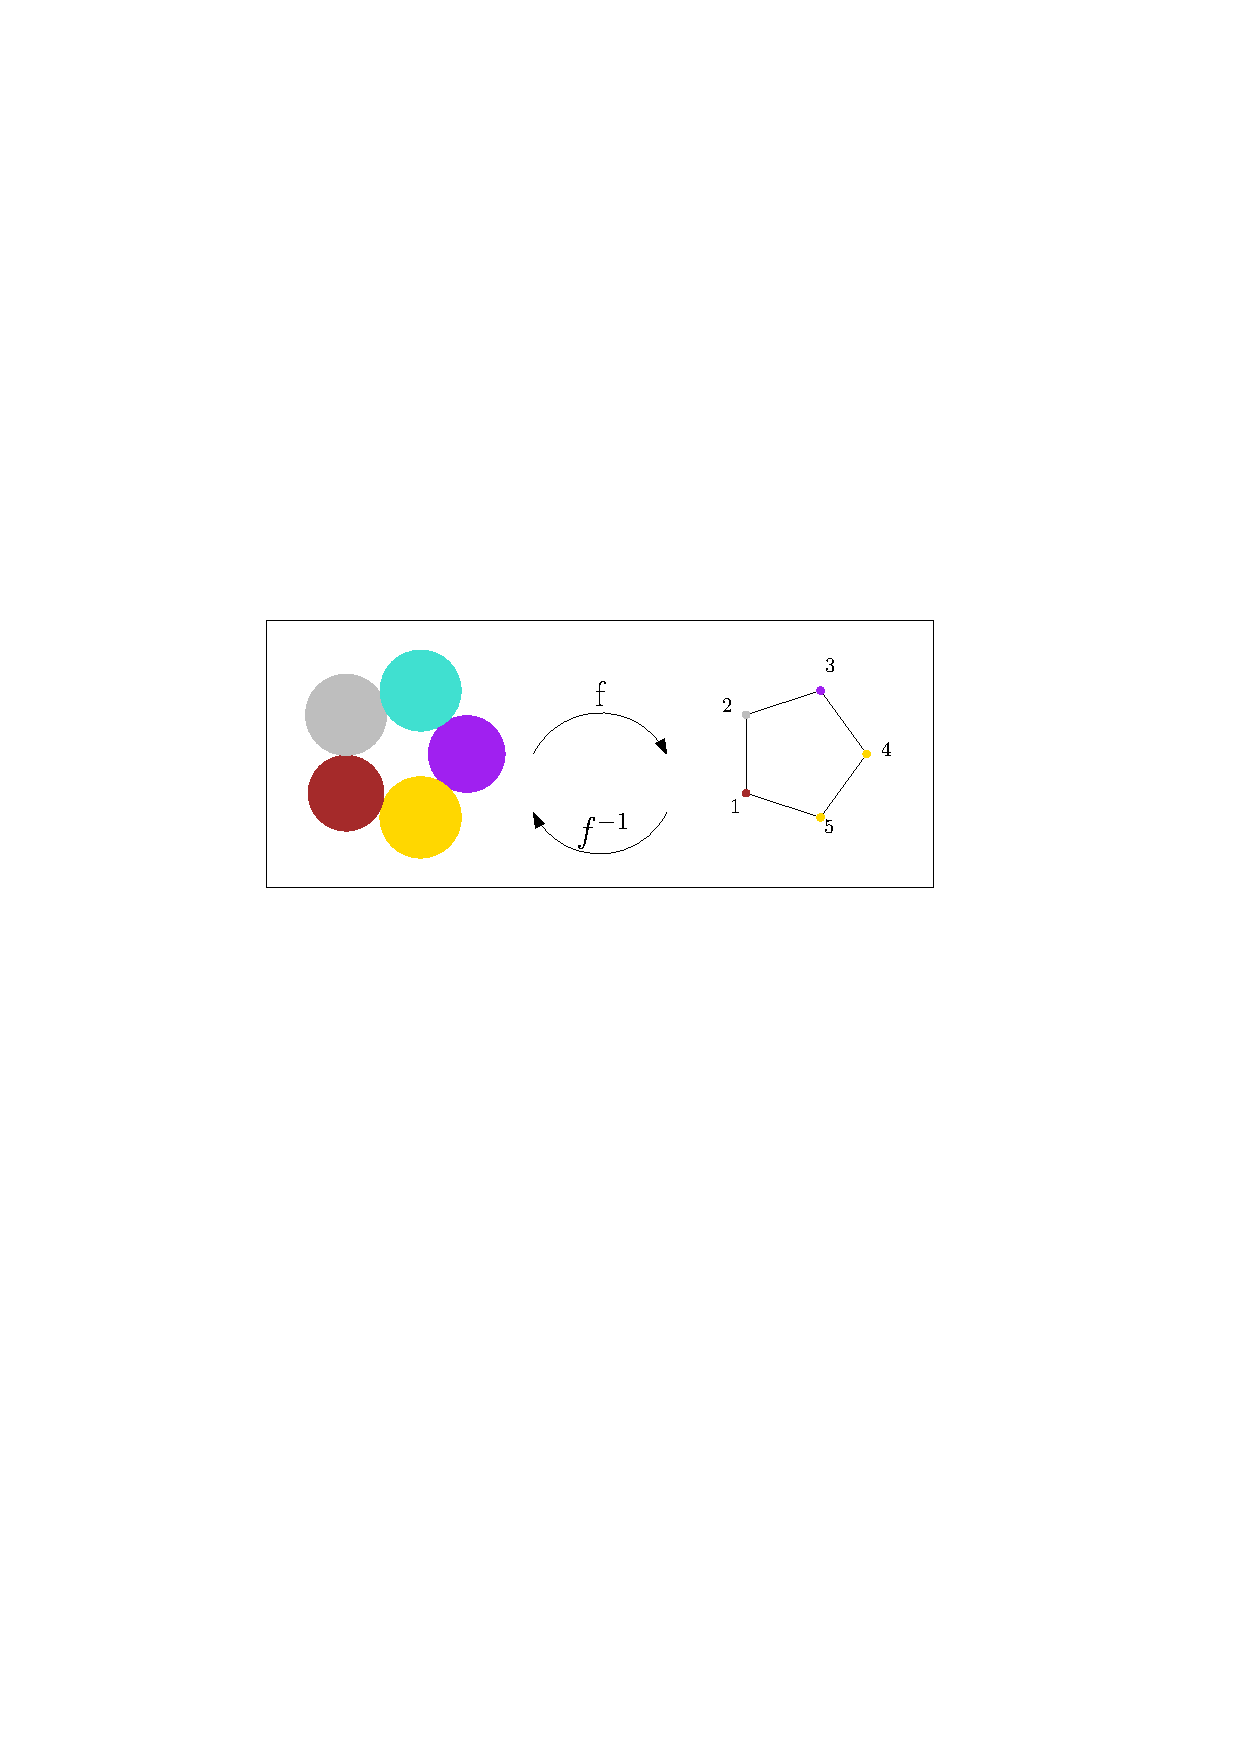
\includegraphics[scale=1]{graphics/diskPackingTheoremExample.pdf}
\end{center} 
\caption{This example represents a disk arrangement and its contact graph.}
%Figure shows a 5-cycle with a unique realization of a disk arrangement.
\label{fig:DiskArrangement-1}
\end{figure}
A \textit{contact graph} $G=(V,E)$ corresponding to a given disk arrangement where there is a bijection $b_V: V \mapsto D$ and a bijection that maps an edge $e_{i,j} \in E$ to an interior disjoint pair of disks $d_i$, $d_j \in D$ (see Figure \ref{fig:DiskArrangement-1}).
Given a disk arrangement, the contact graph can be thought of as a linkage because the distance between two kissing disk equal the sum of radii.  
However if the two disks don't kiss, the distance between their centers is strictly greater than the sum of their radii.
Given a disk arrangement, the contact graph can be thought of as a linkage because the distance between two kissing disk equal the sum of radii.  
However if the two disks don't kiss, the distance between their centers is strictly greater than the sum of their radii.

Koebe's theorem states that for every planar graph $G$, there exists a planar disk arrangement whose contact graph is $G$ \cite{koebe1936kontaktprobleme}.
This motivates the question of whether a planar graph $G$ is a contact graph of a disk arrangement with given radii.
The radii can be given by a weight function.
Let $\omega: V \mapsto \bbR^+$ be the \textit{weight function}.  
$\omega$ assigns a weight to each vertex in $V$.  
Let $\Pi:V \mapsto \bbr^2$ be that planar mapping of vertices.
%$D$ \textit{respects radii assignments} if for every $v \in V$ such that $b_V(v) = D_v$, $\omega(v)$ is the radius of $D_v$.    
%$D$ \textit{respects center assignments} if for every $v \in V$, $\Pi(v)$ is the center of $D_v$.  
%Note that if $\omega$ respects radii assignments, then it can be equivelently said that the linkage $(G,\ell)$ with length assignment $\ell$ also respects radii assignments.  
%In this thesis, unless otherwise stated we assume that the contact graph associates to an $\omega$ and $\Pi$ mapping that respect radii and center assignments.
%we may also interchange contact graph with linkage.



% For the sake of simplicity, throughout this thesis we often refer to disks and their corre- sponding vertices synonymously. For example, we might simply say ’we create a disk D2 with radius r2 that touches disk D1’ instead of saying ’we create a vertex v2, a correspond- ing disk D2 with radius r2 and an edge between v2 and vertex v1 whose corresponding disk is D1’.
% Let G = (V, E) be a graph. We say that G has a realization as a disk intersection (touching) graph, if there exist a set of disks V and a bijection from V to V such that G = (G,V) is a disk intersection (touching) graph. In this case, we say G realizes G. Let Dv ∈ V be the disk of G corresponding to vertex v for any v ∈ V . A radius assignment for G is a function r : V → R+ that assigns a positive real number to each vertex of G. If the radius of disk Dv ∈ V is equal to r(v) for every v ∈ V , then G is said to respect r. A seed assignment for G is a function σ : V → R2 that assigns a point in the plane to each vertex ofG.Ifσ(v)∈Dv foreveryv∈V,thenGissaidtorespectσ.LetΓbeacombinatorial embedding for G. If G is a disk touching graph and if the cyclic order of disks touched by Dv corresponds to the cyclic order of edges incident to the vertex v for any v ∈ V , then G is said to respect Γ.
% %By Koebe's Theorem, every disk arrangement embedded in the plane has a contact graph.
% A \textit{contact graph} represents vertices as interior disjoint disks and by representing edges as as points of intersections (contact), \textit{kissing points} between two disks.  
% The graph corresponding to a given disk arrangement, $\DD$, is said to be the \textit{contact graph}. 
% An ordered disk arrangement preseves the  cyclic order of neighborings disks. 
% %A \it{disk arrangement} is a set, $\DD$, of pairwise interior-disjoint disks in the plane, 
% %$\DD=\left\lbrace C_i \right\rbrace_{i = 1}^n $.


%What is not obvious is when given a graph with positive weights, does there exist a planar drawing?
%Some variants of these problems were known to be NP-Hard.
For planar graphs with positive weighted vertices, we pose two realizability problems:
\begin{prob}[Unordered Realizibility Problem for a Contact Graph]\label{problem:UnorderedContactGraph}
Given a planar graph with positive weighted vertices, is it a contact graph of some disk arrangement where the radii equal the vertex weights?
\end{prob}
\begin{prob}[Ordered Realizibility Problem for a Contact Graph]\label{problem:OrderedContactGraph}
Given a planar graph with positive weighted vertices and a combinatorial embedding, is it a contact graph of some disk arrangement where the radii equal the vertex weights and the counter-clockwise order of neighbors of each disk is specified by the combinatorial embedding?
\end{prob}

An instance of Problem \ref{problem:UnorderedContactGraph} is shown in Figure \ref{fig:DiskArrangement-1} where the cycle graph $C_5$ is the contact graph of unit disks.
It is not difficult to see that there exists a planar graph with positive weights with no realizable disk arrangement.
Consider the a star graph with 6 leafs, each vertex with unit weight.
In any realization, the angle between two consecutive edges must be greater than $\frac{\pi}{3}$. 
The sum of 6 angles is $2 \pi$ however, the sum of 6 consecutive angles is greater than $2\pi$.
The contradiction shows that no realization is possible (refer to Figure \ref{figure:starweel}).
Note that with the wheel graph $W_7$ is realizable as a contact graph of unit disks.

Every path with arbitrary positive radii is realizable as a contact graph, place the vertices on a line.
We show that not all binary trees are realizable, even with unit disks.% of unit radii.
Consider the balanced binary trees of depth $i$ $\left\lbrace T_i \right\rbrace_{i=1}^\infty$ with unit weights on the vertices (see Figure \ref{fig:circlePacking-1}).
These trees are not realizable for sufficiently large $i$.
\begin{figure}[!htbp]\label{fig:circlePacking-1}
\begin{center}
    %add desired spacing between images, e. g. ~, \quad, \qquad etc.
    %(or a blank line to force the subfigure onto a new line)
  \begin{subfigure}[b]{0.21\textwidth}
	  \includegraphics[width=\textwidth]{graphics/BinaryTree1.pdf}
	  \caption{Binary tree $T_2$.}
	  \label{fig:circlePacking1-1}
  \end{subfigure}
  \begin{subfigure}[b]{0.21\textwidth}
	  \includegraphics[width=\textwidth]{graphics/BinaryTree2.pdf}
	  \caption{Binary tree $T_3$.}
	  \label{fig:circlePacking1-2}
  \end{subfigure}
  \begin{subfigure}[b]{0.21\textwidth}
	  \includegraphics[width=\textwidth]{graphics/BinaryTree3.pdf}
	  \caption{Binary tree $T_4$.}
	  \label{fig:circlePacking1-3}
  \end{subfigure}
  \begin{subfigure}[b]{0.21\textwidth}
	  \includegraphics[width=\textwidth]{graphics/BinaryTree4.pdf}
	  \caption{Binary tree $T_5$.}
	  \label{fig:circlePacking1-4}
  \end{subfigure}
  \caption{ We show the linkages $T_2$ through $T_5$ with distance 2 between adjacent vertices.  }
\end{center} 
\end{figure}
%To show that as $i \rightarrow \infty$, the corresponding disk arrangement will not have a drawing.  
%We construct the disk arrangement as follows: (1) place a disk of unit radius centered at origin; (2) for each disk continue to add two non-intersecting kissing disks of unit radius to it.  
%To illustrate, see Figure \ref{fig:circlePacking-1}:
Let $i$ be a positive integer and suppose that $T_i$ is a contact graph of unit disks.
The balanced binary tree $T_i$ has $2^i -1$ vertices.
The total area of the disks is $\left( 2^i -1 \right)^2 \cdot \pi$.
We now derive an upper bound for this area.
%Suppose the root of the disk arrangement is centered at origin.
Suppose the disk corresponding to the root of the tree is centered at the origin.
The centers of the disks at level $j$ are at a distance at most $2\cdot (j-1)$ away from the origin.
The centers of all disks are at distance at most $2 \cdot (i -1)$ away from the origin.
All unit disks are contained in a disk of radius $2i-1$ centered at the origin.
The total area of the disks is at most $(2i-1)^2$.
%Let the total area of the disks arrangement be the sum of the areas of the disks. 
A upper bound of the total area of the disk arrangement is the area of the bounding box of the disks.
The upper bound of the 


\begin{figure}[!htpb]\label{fig:circlePacking-2}
\begin{center}
    %add desired spacing between images, e. g. ~, \quad, \qquad etc.
    %(or a blank line to force the subfigure onto a new line)
  \begin{subfigure}[b]{0.24\textwidth}
	  
\includegraphics[width=\textwidth]{graphics/degree2arrangement.pdf}
	  \caption{A disk arrangement with two layers of disks}
	  \label{fig:circlePacking2-1}
  \end{subfigure}
  \begin{subfigure}[b]{0.24\textwidth}
	  
\includegraphics[width=\textwidth]{graphics/degree3arrangement.pdf}
	  \caption{A disk arrangement with three layers of disks}
	  \label{fig:circlePacking2-2}
  \end{subfigure}
  \begin{subfigure}[b]{0.24\textwidth}
	  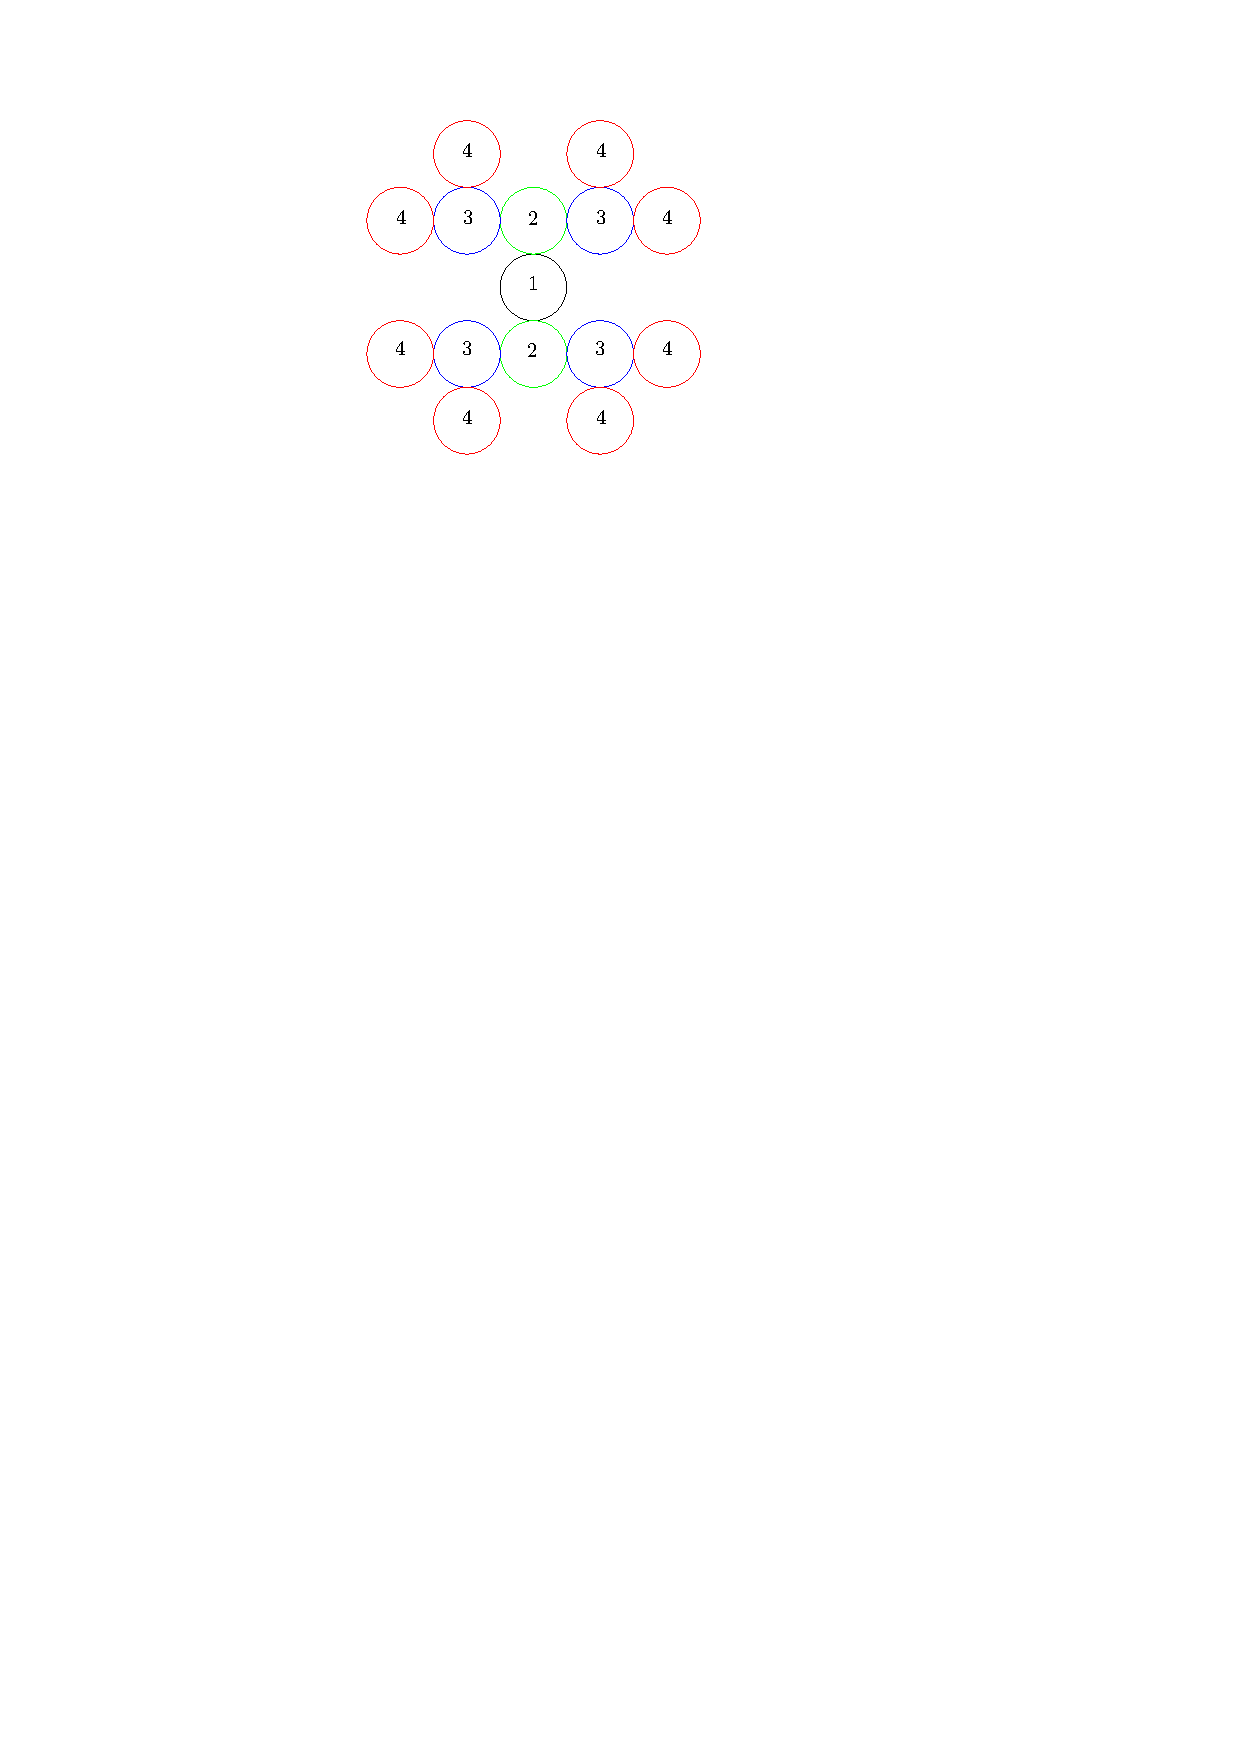
\includegraphics[width=\textwidth]{graphics/degree4arrangement.pdf}
	  \caption{A disk arrangement with four layers of disks}
	  \label{fig:circlePacking2-3}
  \end{subfigure}
  \begin{subfigure}[b]{0.24\textwidth}
	  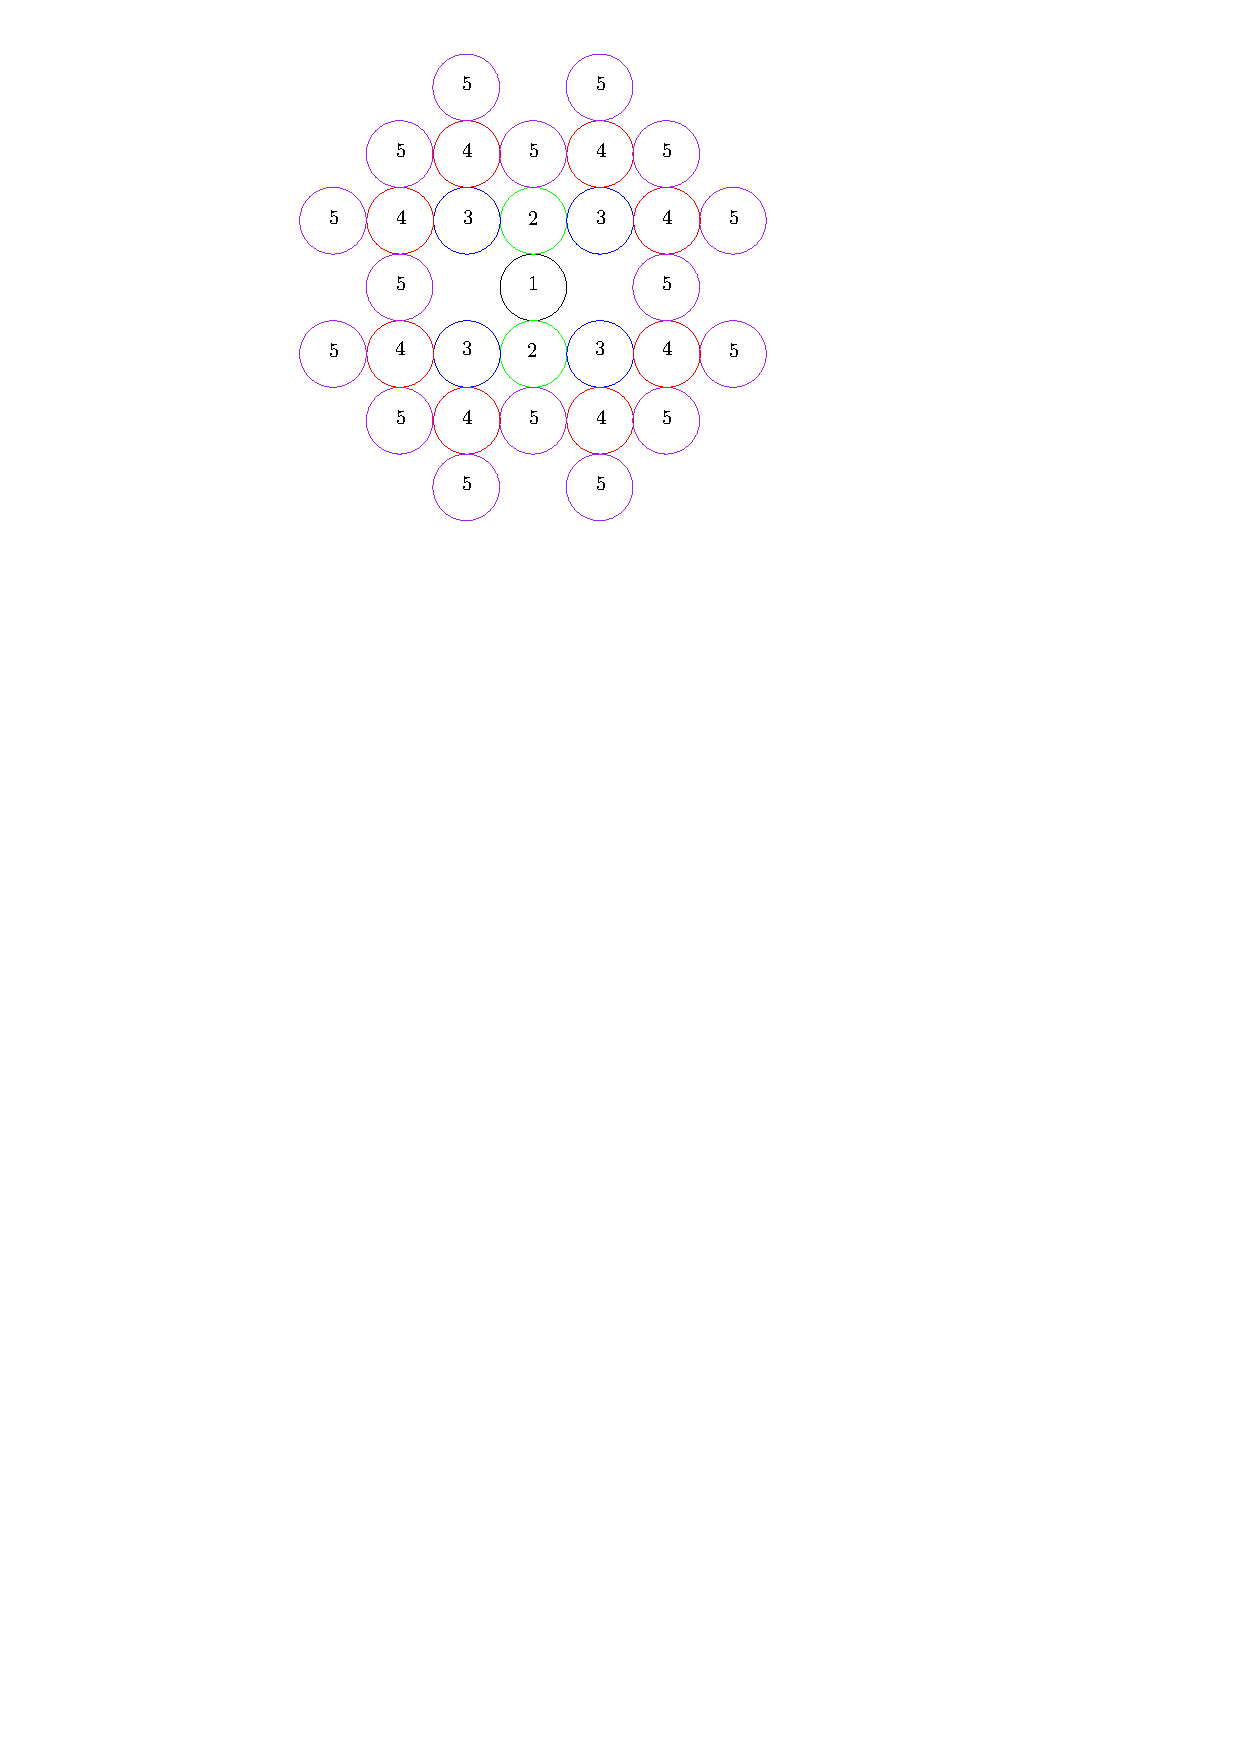
\includegraphics[width=\textwidth]{graphics/degree5arrangement.pdf}
	  \caption{A disk arrangement with five layers of disks}
	  \label{fig:circlePacking2-4}
  \end{subfigure}
\end{center} 
\caption{For $i=2,3,4,5$ the tree $T_i$ is a contact graph of unit disks.}\label{fig:circlePacking-1}
\end{figure}
% The first round has one unit disk.  
% The next round, two unit radii disk are in contact with the first, i.e. Figure \ref{fig:circlePacking1-1}.
% The subsequent rounds are shown in Figures \ref{fig:circlePacking1-2}, \ref{fig:circlePacking1-3}, and \ref{fig:circlePacking1-4}.  
% For each round $i$ we are adding $2^{(i-1)}$ disks, each with an area of $\pi$.  
% The area that the disk arrangement is bounded at round $i$ is a box of length $2\cdot (2\cdot (i-1)+1)$ totalling to an area of $(4\cdot i^2 - 4\cdot i + 1)$.  
% Meanwhile the total area of the disk arrangement at $i$ is $\pi \cdot (2^i - 1)$.  The exponential growth rate of the disk packing will exceed its bounded area for sufficiently large $i$, i.e. pick $i \geq 6$.
Figure \ref{fig:circlePacking-2} shows the first four non-trivial trees as a contact graph of unit disks.
Every disk at level up to $i$ is contained in a disk of radius $2\cdot i - 1$ centered at the origin.
The total area of the disk arrangement is $(2\cdot i -1)^2 \cdot \pi$. 
When $i\geq 8$ we have a contradiciton.%the total area of the disk arrangement exceeds the total bounded area and thus we have a contradiction.

\begin{figure}[!htbp]\label{fig:circlePacking-3}
\begin{center}
    %add desired spacing between images, e. g. ~, \quad, \qquad etc.
    %(or a blank line to force the subfigure onto a new line)
  \begin{subfigure}[b]{.48\textwidth}
  \begin{center}
	  \includegraphics[scale=.9]{graphics/OrderedDiskArrangementExample1.pdf}
	  \label{fig:circlePacking3-1}
	  \end{center}
  \end{subfigure}
  \begin{subfigure}[b]{0.48\textwidth}
  \begin{center}
	  \includegraphics[scale=.9]{graphics/OrderedDiskArrangementExample2.pdf}	  
	  \label{fig:circlePacking3-2}
	  \end{center}
  \end{subfigure}
  \caption{Consider these two ordered disk arrangements where A and B are in the concentric rings of disks.  The large disks are in contact to A and B respectively.  
  If A and B are adjacent, then there is a restriction of how large the size of the disks can be that are attached to them as seen in on the left.  
  Whereas if A and B are not adjacent in this disk arrangment as shown on the right, the size of the kissings disks could be arbitrarily large.}
\end{center} 
\end{figure}

There are instances where a planar graph with weights admits a realization but the cyclic order of neighbors may not be the same as the combinatorial embedding.
Define $G$ as follows: start with a star centered at $C$ and with 6 leafs, $A_1$ through $A_6$; attach two leafs, $B_1$ and $B_2$, to $A_1$ and  $A_2$ respectively (see  Figure \ref{fig:circlePacking-3}).
Let the weight of $C$ be $1+\epsilon$ for sufficiently small $\epsilon > 0$.
The neighbors of $C$ have unit weight.
The weights of the two leaves have weight $\frac{1}{\epsilon}$/
The right of Figure \ref{fig:circlePacking-3}) shows a realization where $A_1$ and $A_2$ are in opposite position of the counter-clockwise order around $C$.
If $A_1$ and $A_2$ are required to be consecutive in the counter-clockwise order around $C$, there is no realization.
%as epsilon goes to 0 the half planes approximates the disks and so the disks will intersect as well.  label everything, draw halff planes, epsilon and delta, 1/epsilon.

Suppose there is a realization where $A_1, \ldots, A_6$ are in the counter-clockwise order around $C$ (see Figure \ref{{fig:DiskArrangement-4}}).
If $\epsilon>0$ is sufficiently small, then the centers of of $A_1, \ldots, A_6$ are arbitrarily close to the vertices of a regular hexagon.
Consider the common tangent lines between $A_1$ and $B_1$ and $A_2$ and $B_2$.
The possible position of tangent line between $A_1$ and $B_1$ ranges from the common tangent line of $A_1$ and $A_6$ to the common tangent line of $A_1$ and $A_2$.
Similarly, The possible position of tangent line between $A_2$ and $B_2$ ranges from the common tangent line of $A_2$ and $A_3$ to the common tangent line of $A_1$ and $A_2$.
In any position, the common tangent lines between $A_1$ and $B_1$ and $A_2$ and $B_2$ intersect.
If $\frac{1}{\epsilon}$ is sufficiently large, then the disks $D_1$ and $D_2$ also intersect.
This contradicts that there is a realization.
\begin{figure}[!hbtp]
\begin{center}
\includegraphics[scale=1]{graphics/orderedPlaneIntersection.pdf}
\end{center} 
\caption{This example represents a disk arrangement and its contact graph.}
%Figure shows a 5-cycle with a unique realization of a disk arrangement.
\label{fig:DiskArrangement-4}
\end{figure}
Figure \ref{fig:circlePacking-3} shows how an ordered contact graph may not be realizable.  
On the left, it shows a limitation on the weights of the disks that are in contact with disks A and B. 
On the right, the figure shows the order where A and B are on opposing ends of the ring of disks and can allow of arbitrary size of wieghted disks in contact with A and B.
% Figure \ref{fig:orderedFaces.pdf} shows three polygons with a common hinge.
% In the counter-clockwise order $(A,B,C)$, the polygonal linkage admits a realization whereas in the counter-clockwise order $(A,C,B)$, it does not admit a realization.
% \subsection{Disk Packing Confinement Problem}

% Given inputs of radii 
% By adding constraints to the embeddings of disk arrangements, we can devise realizability problem 
% by a volume argument.
% \begin{enumerate}%1,2,3,4....
% \item Round 1: Start with a disk of unit radius.
% \item Round 2: Add two kissing disks, each of diameter 2, that do not intersect with any other 
% disk (they 
% may kiss other
% disk).
% \item Round 3 and Higher: For each new kissing disk added, add two more non-intersecting kissing 
% disks of diameter 2 to it.
% \end{enumerate} 


% Figure (\ref{fig:circlePacking-1}) illustrates the iterative problem.  The problem with this is that 
% the area in
% which is necessary to contain this disk growing disk arrangement will exceed the area needed to 
% contain it.





%The corresponding intersection graph of a disk packing is a graph whose vertices are the disks and edges correspond to two disks that contact each other.
% \section{Disk Arrangements}
% It turns out the disk arrangements are an equivalent way to to represent plane graphs.  By 
% representing vertices as interioir disjoint disks and by representing edges as as points of 
% intersections (contact), \textit{kissing 
% points} between two disks.  The graph corresponding to a given disk arrangement, $\DD$, is said to 
% be the \textit{contact graph}. A \it{disk arrangement} is a set, $\DD$, of pairwise 
% interior-disjoint disks in the plane, 
% $\DD=\left\lbrace C_i \right\rbrace_{i = 1}^n $.
% $\left\lbrace C_i \right\rbrace_{i = 1}^n $ such that for any circle $C \in \left\lbrace C_i 
% \right\rbrace_{i = 1}^n$, $C$


% %(fig 1) a disk arrangement
% %(fig 2) an equivalent contact graph to (fig 1)
% A classical result by Thurston and Koebe is that every disk arrangement embedded into the plane had 
% a corresponding plane graph.
% \begin{thm}[\ref{stephenson2005introduction}Disk Packing Theorem]\label{thm2-1}
% For every graph $G$, there is a disk arrangement in the
% plane whose contact graph is isomorphic to $G$.
% \end{thm}

% %add a paragraph with atoms of molecules are modeled with disks and balls of fixed radii. The 
% %if two disks are in contact, then the  distance between their centers  = the sum of the radii
% %conclude: disk arrangements are better models for representing atoms and molecules fixed distance 
% % betweeen atoms
% \begin{prop}
%  For every linkage $L$, there is a disk arrangement in the
% plane whose contact graph is isomorphic to $L$.
% \end{prop}



% \begin{enumerate}%1,2,3,4....
% %\item Introduce the circle packing theorem.
% \item Show the relation between polygonal linkages and disk arrangengements.
% \end{enumerate} 
% % \subsubsection{Ordered Disk Arrangement}
% Suppose we're given a tree. By the disk packing theorem we can ascertain a sense of order for the 
% isomorphic disk packing.  An \textit{ordered disk arrangement} is a rooted tree in which the 
% counter-clockwise ordering of adjacent vertices.
% % 


% The embedding problems for trees and corresponding disk arrangements are as follows:
% \begin{prob}[Unordered Realizibility Problem for the Tree]\label{problem:UnorderedContactGraph}
% For a tree with positive weights for the verticies, it asks whether it is a contact graph of some 
% disk arrangement where the radii are equal to the vertex weights.
% \end{prob}

% \begin{prob}[Ordered Realizibility Problem for the Tree]\label{problem:OrderedContactGraph}
% For a tree with positive weights for the vertices, it asks whether its corresponding graph is the 
% ordered contact graph of some disk arrangement where the radii equal the vertex weights.
% \end{prob}
